\documentclass{article}

\usepackage{graphicx}
\usepackage{tikz}
\usepackage{tikzsymbols}
\usetikzlibrary{calc,patterns,shapes.geometric}
\pagestyle{empty}
\usepackage[margin=0pt]{geometry}
\geometry{papersize={14in,12in}}

\def\centerarc[#1](#2)(#3:#4:#5){\draw[#1] ($(#2)+({#5*cos(#3)},{#5*sin(#3)})$) arc (#3:#4:#5);}

\begin{document}
	\begin{figure}
		\centering
		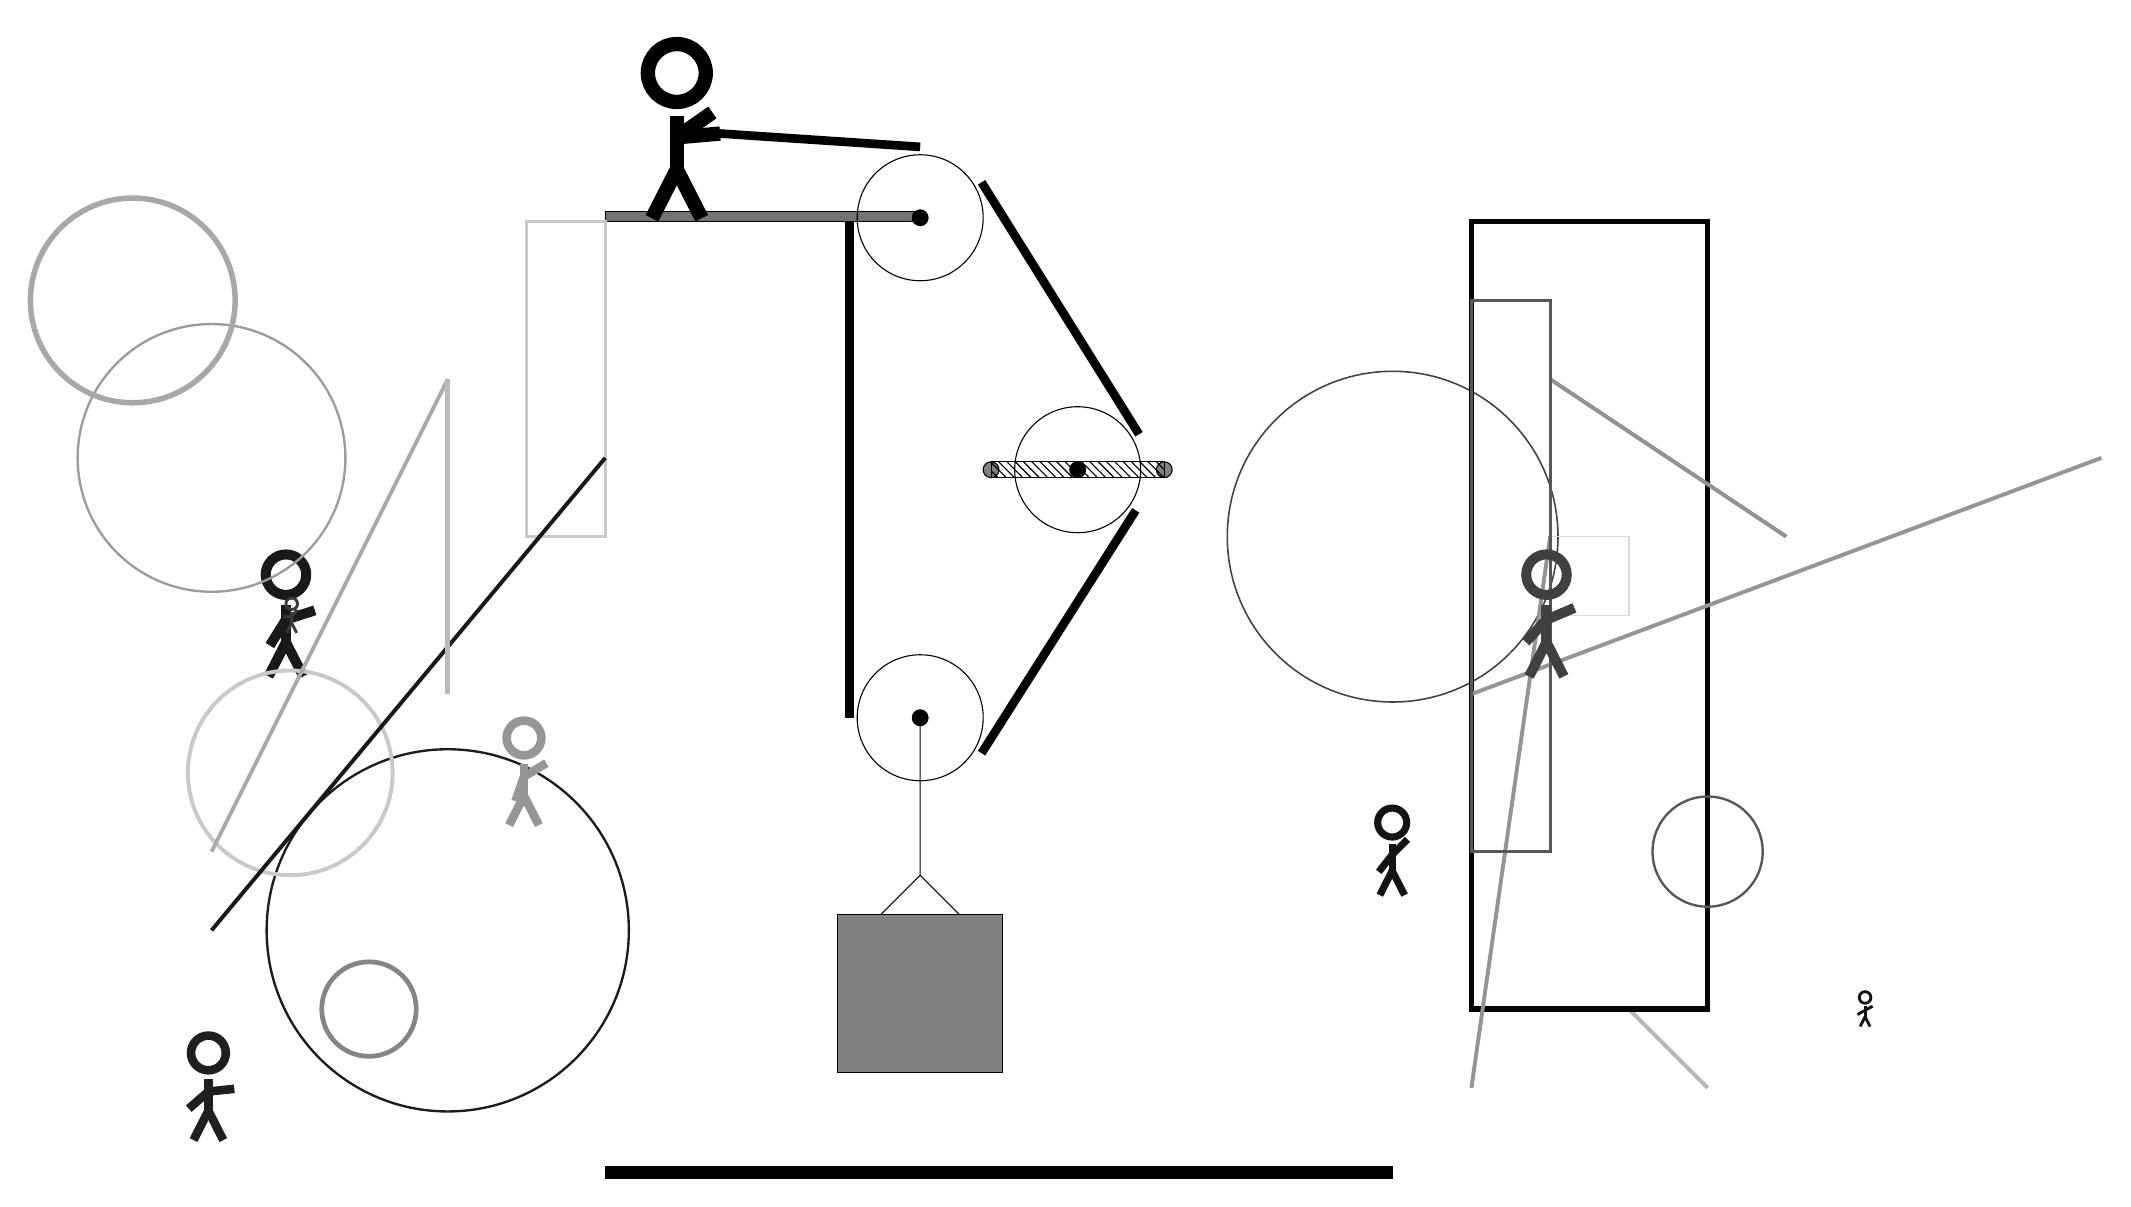
\begin{tikzpicture}
			%%%%% START %%%%%
			
			\draw[fill=black!55] (-2, 9) rectangle (2, 9.125);
			
			\draw (2, 2.7) circle (0.8);
			\draw[fill=black] (2, 2.7) circle (0.1);
			
			\draw (2, 9.05) circle (0.8);
			\draw[fill=black] (2, 9.05) circle (0.1);
			
			\draw[fill=white](4, 5.85) circle (0.8);
			\draw[fill=black] (4, 5.85) circle (0.1);
			\draw[fill=black!50] (2.9, 5.85) circle (0.1);
			\draw[fill=black!50] (5.1, 5.85) circle (0.1);
			\draw[pattern=north west lines, pattern color=black] (2.9, 5.95) rectangle (5.1, 5.75);
			
			\draw (2, 2.7) -- (2, 0.7) -- (1.5, 0.2) -- (2.5, 0.2) -- (2, 0.7);
			\draw[fill=black!50] (0.95, 0.2) rectangle (3.05, -1.8);
			
			\node[line width=0.4mm, color=black!90] at (-6, 4) {\Strichmaxerl[7][58][18]};
			
			\draw[line width=0.4mm, color=black!12] (10, 3) rectangle (10, 3);
			\draw[line width=0.5mm, color=black!28](12, -2) -- (11, -1);
			\draw [line width=0.3mm, color=black!39](-7, 6) circle (1.7);
			
			\draw [line width=0.2mm, color=black!74](8, 5) circle (2.1);
			\node[line width=0.2mm, color=black!92] at (8, 1) {\Strichmaxerl[5][52][45]};
			\node[line width=0.7mm, color=black!78] at (-6, 4) {\Strichmaxerl[2][2][51]};
			
			\draw [line width=0.3mm, color=black!89](-4, 0) circle (2.3);
			\draw[line width=0.7mm, color=black!98] (9, -1) rectangle (12, 9);
			\draw[line width=0.4mm, color=black!21] (-2, 5) rectangle (-3, 9);
			
			\draw[line width=0.2mm, color=black!14] (10, 4) rectangle (11, 5);
			
			\draw[line width=0.5mm, color=black!43](13, 5) -- (10, 7);
			\node[line width=0.4mm, color=black!88] at (-7, -2) {\Strichmaxerl[6][41][6]};
			
			\node[line width=0.3mm, color=black!92] at (14, -1) {\Strichmaxerl[2][29][29]};
			\draw[line width=0.5mm, color=black!41](9, 3) -- (17, 6);
			\draw [line width=0.6mm, color=black!48](-5, -1) circle (0.6);
			\node[line width=0.6mm, color=black!41] at (-3, 2) {\Strichmaxerl[6][71][31]};
			
			\draw [line width=0.5mm, color=black!21](-6, 2) circle (1.3);
			\draw [line width=0.3mm, color=black!66](12, 1) circle (0.7);
			\draw [line width=0.7mm, color=black!34](-8, 8) circle (1.3);
			\draw[line width=0.5mm, color=black!42](9, -2) -- (10, 5);
			
			\draw[line width=0.5mm, color=black!90](-2, 6) -- (-7, 0);
			\draw[line width=0.4mm, color=black!66] (9, 8) rectangle (10, 1);
			\draw[line width=0.5mm, color=black!33](-7, 1) -- (-4, 7);
			\node[line width=0.2mm, color=black!75] at (10, 4) {\Strichmaxerl[7][47][23]};
			
			\draw[line width=0.6mm, color=black!27] (-4, 7) rectangle (-4, 3);
			
			
			\draw[line width=1.1mm] (1.1, 9) -- (1.1, 2.7);
			\centerarc[line width=1.1mm](2, 2.7)(180:330:0.9);
			\draw[line width=1.1mm](2.7794, 2.25) -- (4.7373, 5.3338);
			\centerarc[line width=1.1mm](4, 5.85)(390:325:0.9);
			\draw[line width=1.1mm](4.7794, 6.3) -- (2.7794, 9.5);
			\centerarc[line width=1.1mm](2, 9.05)(30:90:0.9);
			\draw[line width=1.1mm](2, 9.95) -- (-1, 10.15);
			
			\node at (-1, 10.15) {\Strichmaxerl[10][-175][35]};
			
			\draw[fill=black] (-2, -3) rectangle (8, -3.15);
			
			%%%%% END %%%%%
		\end{tikzpicture}
	\end{figure}	
\end{document}